\chapter{Court Keypoint Detection and Homography}
\label{ch:court}

% Styles for the canonical court schematic (Fig.~\ref{fig:court-template}) and the
% model-head diagrams, kept local to this chapter.
\tikzset{
  courtline/.style={line width=0.9pt, black!75},
  netline/.style={line width=1.3pt, black!85, dash pattern=on 4pt off 2pt},
  kpt/.style={circle, draw=orange!85!black, fill=orange!85!black,
    inner sep=0pt, minimum size=4.2pt},
  kptlbl/.style={font=\scriptsize\bfseries, text=black!80},
  ctr/.style={rectangle, draw=blue!70!black, fill=blue!70!black,
    inner sep=0pt, minimum size=4.2pt},
  dimarr/.style={{Stealth[scale=0.8]}-{Stealth[scale=0.8]}, line width=0.5pt, blue!55!black},
  dimlbl/.style={font=\scriptsize, text=blue!55!black, fill=white, inner sep=1pt},
}

This chapter applies the protocol of Chapter~\ref{ch:methodology} to the second
perception sub-task, locating the fixed landmarks of the tennis court in a single
broadcast frame and using them to register the image to a court-plane coordinate
system. Where ball tracking must follow a small moving target through time, court
detection faces the opposite problem: the landmarks are static and well defined,
but they must be located precisely, because their pixel coordinates feed a
homography whose accuracy in court metres degrades quickly with keypoint error.
Four heatmap models are compared on the court-keypoint dataset of
Section~\ref{sec:meth-court}, a from-scratch baseline and three models built on
pretrained backbones of very different sizes, and each is scored both by the
keypoint-localisation metrics of Section~\ref{sec:meth-metrics-loc} and by the
geometric registration metrics of Section~\ref{sec:meth-metrics-geom}. The
chapter answers the second research question (RQ2) on which backbone gives the
best accuracy against latency trade-off for fourteen-keypoint court detection,
and whether the chosen model is reliable enough to drive a homography into
court-metric space.

Unlike the ball comparison of Chapter~\ref{ch:ball}, the court comparison is a
single-stage one: all four models were trained and evaluated on the one court
split of Section~\ref{sec:meth-splits-court}, with no separate subset-selection
stage, so the numbers in this chapter are directly comparable across models. The
model carried forward into the integrated system of
Chapter~\ref{ch:integrated} is selected here on the combined evidence of accuracy,
geometric registration quality, throughput, and size.

\section{Task and Data Specifics}
\label{sec:court-task}

Court detection is posed as the localisation of fourteen fixed court landmarks in
a single RGB frame, each landmark predicted as the peak of a dedicated heatmap
channel. The fourteen landmarks follow the ordering of the TennisCourtDetector
collection \cite{yastrebksv2023courtdetector} that the dataset is drawn from, and
that ordering is fixed throughout the data pipeline, the models, and the
geometric template, so it is documented once here. Table~\ref{tab:court-keypoints}
lists the fourteen landmarks together with their coordinates in the canonical
court template described in Section~\ref{sec:court-homography}, and
Figure~\ref{fig:court-template} draws them on a scale court diagram. The four
outer corners (indices~0 to~3) are the doubles-court corners; indices~4 to~7 are
the points where the singles sidelines meet the two baselines; indices~8 to~11
are the points where the singles sidelines meet the two service lines; and
indices~12 and~13 are the centre points of the two service lines, where the
centre service line meets them.

\begin{table}[t]
  \centering
  \small
  \setlength{\tabcolsep}{6pt}
  \caption{The fourteen annotated court keypoints in the TennisCourtDetector
    ordering used throughout the court pipeline, with their coordinates in the
    canonical court template of Section~\ref{sec:court-homography}. The template
    origin is the court centre, the $x$ axis runs along the court width towards
    the right sideline, and the $y$ axis runs along the court length towards the
    top baseline; all coordinates are in metres. A fifteenth heatmap channel
    (the court centre) is constructed rather than annotated, as described in the
    text.}
  \label{tab:court-keypoints}
  \begin{tabular}{r l r r}
    \toprule
    Index & Landmark & $x$ (m) & $y$ (m) \\
    \midrule
    0  & top-left outer (doubles) corner       & $-5.485$ & $+11.885$ \\
    1  & top-right outer (doubles) corner      & $+5.485$ & $+11.885$ \\
    2  & bottom-left outer (doubles) corner    & $-5.485$ & $-11.885$ \\
    3  & bottom-right outer (doubles) corner   & $+5.485$ & $-11.885$ \\
    4  & top-left singles baseline corner      & $-4.115$ & $+11.885$ \\
    5  & bottom-left singles baseline corner   & $-4.115$ & $-11.885$ \\
    6  & top-right singles baseline corner     & $+4.115$ & $+11.885$ \\
    7  & bottom-right singles baseline corner  & $+4.115$ & $-11.885$ \\
    8  & top-left service-line point           & $-4.115$ & $+6.400$ \\
    9  & top-right service-line point          & $+4.115$ & $+6.400$ \\
    10 & bottom-left service-line point        & $-4.115$ & $-6.400$ \\
    11 & bottom-right service-line point       & $+4.115$ & $-6.400$ \\
    12 & top centre service point              & $\phantom{+}0.000$ & $+6.400$ \\
    13 & bottom centre service point           & $\phantom{+}0.000$ & $-6.400$ \\
    \bottomrule
  \end{tabular}
\end{table}

\begin{figure}[t]
  \centering
  \begin{tikzpicture}[scale=0.5]
    % court drawn with the length (y, 23.77 m) along the horizontal screen axis
    % and the width (x, 10.97 m) along the vertical screen axis, for compactness.
    % screen = (court_y, court_x).
    % outer doubles rectangle
    \draw[courtline] (-11.885,-5.485) rectangle (11.885,5.485);
    % singles sidelines
    \draw[courtline] (-11.885,-4.115) -- (11.885,-4.115);
    \draw[courtline] (-11.885, 4.115) -- (11.885, 4.115);
    % service lines
    \draw[courtline] (6.40,-4.115) -- (6.40,4.115);
    \draw[courtline] (-6.40,-4.115) -- (-6.40,4.115);
    % centre service line
    \draw[courtline] (-6.40,0) -- (6.40,0);
    % net
    \draw[netline] (0,-5.485) -- (0,5.485);
    \node[dimlbl] at (0,5.95) {net};
    % keypoints (index : screen coords = (court_y, court_x))
    \foreach \i/\y/\x in {%
        0/11.885/-5.485, 1/11.885/5.485, 2/-11.885/-5.485, 3/-11.885/5.485,
        4/11.885/-4.115, 5/-11.885/-4.115, 6/11.885/4.115, 7/-11.885/4.115,
        8/6.40/-4.115, 9/6.40/4.115, 10/-6.40/-4.115, 11/-6.40/4.115,
        12/6.40/0, 13/-6.40/0} {
      \node[kpt] (k\i) at (\y,\x) {};
    }
    % index labels, placed to avoid the lines
    \node[kptlbl, above left=0pt of k0] {0};
    \node[kptlbl, above right=0pt of k1] {1};
    \node[kptlbl, below left=0pt of k2] {2};
    \node[kptlbl, below right=0pt of k3] {3};
    \node[kptlbl, below=1pt of k4] {4};
    \node[kptlbl, above=1pt of k5] {5};
    \node[kptlbl, above=1pt of k6] {6};
    \node[kptlbl, below=1pt of k7] {7};
    \node[kptlbl, above left=-1pt of k8] {8};
    \node[kptlbl, above right=-1pt of k9] {9};
    \node[kptlbl, below left=-1pt of k10] {10};
    \node[kptlbl, below right=-1pt of k11] {11};
    \node[kptlbl, above right=0pt of k12] {12};
    \node[kptlbl, below right=0pt of k13] {13};
    % court centre channel
    \node[ctr] (c) at (0,0) {};
    \node[dimlbl, below right=-1pt of c] {centre};
    % dimensions
    \draw[dimarr] (-11.885,-6.4) -- (11.885,-6.4);
    \node[dimlbl] at (0,-6.4) {$23.77$ m (length)};
    \draw[dimarr] (12.9,-5.485) -- (12.9,5.485);
    \node[dimlbl] at (12.9,0) {$10.97$ m};
    \draw[dimarr] (-12.9,-4.115) -- (-12.9,4.115);
    \node[dimlbl] at (-12.9,0) {$8.23$ m};
    \draw[dimarr] (0,4.7) -- (6.40,4.7);
    \node[dimlbl] at (3.2,4.7) {$6.40$ m};
  \end{tikzpicture}
  \caption{The canonical tennis court template and the fourteen annotated
    keypoints, drawn to scale with the court length along the horizontal axis for
    compactness. Orange discs mark the fourteen annotated landmarks of
    Table~\ref{tab:court-keypoints}, numbered by their channel index; the blue
    square at the centre marks the constructed fifteenth channel. The dashed line
    is the net. Dimensions are the International Tennis Federation court
    specification: a doubles court of $23.77 \times 10.97$ m, a singles width of
    $8.23$ m, and service lines $6.40$ m from the net.}
  \label{fig:court-template}
\end{figure}

The dataset is the publicly distributed TennisCourtDetector collection introduced
in Section~\ref{sec:meth-court}, and Figure~\ref{fig:court-gt} there shows two
annotated frames. Its split is the deterministic, seedless partition of
Section~\ref{sec:meth-splits-court}: the 6\,630 training records are used as
supplied, and the 2\,211 validation records are sorted by identifier and divided
into 1\,105 validation records and the remainder for test. 

\section{Preprocessing and Learning Targets}
\label{sec:court-preproc}

Every frame is resized to a fixed $360 \times 640$ input (height by width), and the predicted keypoints are
scaled back to the original frame resolution for evaluation. The original frames
of this dataset are $1280 \times 720$, so the rescaling factor from the input
back to the original is uniform at a factor of two on each axis; this factor
matters for the strict-tolerance results and is taken up again in
Section~\ref{sec:court-analysis}. Pixel intensities are always divided by 255 to
lie in $[0, 1]$, and for the three models built on ImageNet-pretrained backbones
the per-channel ImageNet mean and standard deviation are additionally subtracted
and divided, so that the inputs match the statistics the backbones were
pretrained on; the from-scratch baseline uses the plain $[0, 1]$ scaling only.

The learning target for each annotated keypoint is a CenterNet-style Gaussian
blob centred on the landmark \cite{zhou2019centernet}, rendered into that
keypoint's heatmap channel at the model's output resolution.

Data augmentation is applied to the training split only. It changes brightness
by up to $\pm 0.3$ of the intensity range, scales contrast by a factor drawn from
$[0.7, 1.3]$, and with probability one half flips the frame horizontally. As in
the ball pipeline, the horizontal flip is the augmentation that interacts with the
labels, and it does so more complicatedly here than for a single ball: flipping the
image left to right not only remaps each keypoint x-coordinate to $W - 1 - x$ but
also rearrange the keypoint indices, because a left landmark becomes a right
landmark. The permutation swaps the symmetric left and right pairs (the two outer
corners, the two singles baseline corners, the singles points, and the service
points) while leaving the two centre service points unchanged, and it is applied
as a fixed index map so that each channel continues to predict the correct
landmark after the flip.

\section{Models}
\label{sec:court-models}

Four models are compared, chosen to span the design space from a faithful
reimplementation of the dataset's own baseline to backbones of widely differing
capacity and cost. All four take a single RGB frame and emit a fifteen-channel
heatmap, and all four are trained under the identical regime described below, so
that the comparison isolates the effect of the backbone and the output
resolution. Table~\ref{tab:court-models} summarises them along the axes that
shape the results.

\begin{table}[t]
  \centering
  \small
  \setlength{\tabcolsep}{5pt}
  \caption{The four court-keypoint models. All emit a fifteen-channel heatmap
    (fourteen landmarks plus the constructed centre). Output stride is the ratio
    of the input resolution to the heatmap resolution: the two stride-1 models
    predict at the full $360 \times 640$ input grid, the two stride-4 models at a
    $90 \times 160$ grid. Parameter counts are computed from the implementations
    used here.}
  \label{tab:court-models}
  \begin{tabular}{@{}l p{3.5cm} p{3.2cm} c c c r@{}}
    \toprule
    Model & Backbone & Decoder / head & \makecell{Out.\\stride} & \makecell{Gauss.\\radius}
          & \makecell{ImageNet\\norm.} & \makecell[r]{Params\\(M)} \\
    \midrule
    TrackNet-court & VGG-style encoder-decoder(from scratch) & transposed-conv decoder with skips & 1 & 15 & no  & 20.8 \\
    ResNet50       & ResNet-50(ImageNet)                      & three transposed-conv blocks       & 4 & 8  & yes & 34.0 \\
    HRNet          & HRNet-W32(timm features)                 & stride-4 feature tap + $1\times1$  & 4 & 8  & yes & 30.9 \\
    MobileNetV3    & MobileNetV3-Small(ImageNet)              & U-Net decoder                       & 1 & 15 & yes & 1.28 \\
    \bottomrule
  \end{tabular}
\end{table}

TrackNet-court is a faithful reimplementation of the baseline shipped with the
dataset \cite{yastrebksv2023courtdetector}, the same VGG-style encoder-decoder
backbone used for ball tracking in Chapter~\ref{ch:ball}
\cite{huang2019tracknet}, adapted to take a single three-channel frame rather
than a stacked window and to emit fifteen channels rather than one. Its decoder
upsamples back to the full input resolution through transposed convolutions with
skip connections, so it predicts at output stride one, a $360 \times 640$ heatmap
per channel, and it is the only model trained from scratch without ImageNet
normalisation.

ResNet50 pairs an ImageNet-pretrained ResNet-50 backbone \cite{he2016resnet} with
the simple-baseline pose decoder of Xiao et al.~\cite{xiao2018simplebaselines}:
three transposed-convolution blocks that upsample the stride-32 backbone features
to a stride-4 heatmap, followed by a $1 \times 1$ convolution to fifteen channels.
It predicts at output stride four, a $90 \times 160$ heatmap, and it is the
heaviest model at thirty-four million parameters.

HRNet is built on an HRNet-W32 backbone. It should be noted that the implementation taps a
stride-4 feature map from the backbone's feature pyramid and applies a
$1 \times 1$ convolutional head, rather than using HRNet's native
full-resolution branch; it is therefore a stride-4 model in the same sense as
ResNet50, and this design choice bears directly on its strict-tolerance accuracy,
as Section~\ref{sec:court-analysis} discusses. It carries thirty-one million
parameters.

MobileNetV3 pairs an ImageNet-pretrained MobileNetV3-Small backbone
\cite{howard2019mobilenetv3}, the efficient inverted-residual architecture in the
MobileNet line \cite{sandler2018mobilenetv2}, with a U-Net-style decoder that
upsamples all the way back to the full input resolution. It therefore predicts at
output stride one, a $360 \times 640$ heatmap, like TrackNet-court, but at a
fraction of the size: at 1.28 million parameters it is roughly one sixteenth the
size of TrackNet-court and one twenty-fifth the size of ResNet50.

All four models output raw logits, with the sigmoid applied inside the loss and
at evaluation. They were trained with a common recipe, the Adam optimiser
\cite{kingma2015adam} with a CenterNet-style penalty-reduced focal loss on the
sigmoid of the predicted heatmaps \cite{zhou2019centernet}, which drives the
response towards one at each keypoint peak while reducing the penalty on the
pixels around it in proportion to their Gaussian target value, a learning rate of
$10^{-4}$ halved on plateau, a batch size of eight, and early stopping with a
patience of thirty epochs. The checkpoint kept for each model is the one with the best validation
accuracy at the seven-pixel tolerance, measured in the resized input space; the
distinction between that monitoring metric and the test metric reported below is
discussed in Section~\ref{sec:court-analysis}. A keypoint coordinate is decoded
from a predicted heatmap by locating the peak channel response, refining it to
sub-pixel precision with a local three-by-three intensity-weighted mean, and
scaling by the output stride and the input-to-original factor; a peak below a
confidence threshold of 0.3 return the no-keypoint.

\section{Homography Estimation}
\label{sec:court-homography}

The motivation for detecting court keypoints precisely is that they anchor a
planar homography, the map from image pixels $(u, v)$ to court-plane coordinates
$(X, Y)$ in metres that turns a detected ball position into a measurement on the
court and so makes a in-or-out decision possible. The court is planar
and the camera projection is perspective, so the image-to-court map is a single
$3 \times 3$ homography. The canonical court template against which the homography
is fitted is the metric layout of Table~\ref{tab:court-keypoints} and
Figure~\ref{fig:court-template}: a doubles court of $23.77 \times 10.97$ m with
the origin at the court centre, built directly from the International Tennis
Federation court dimensions, the singles width of $8.23$ m and the service lines
$6.40$ m from the net.

The homography is estimated from the detected keypoints with a
random-sample-consensus fit, known as RANSAC \cite{fischler1981ransac}, which is essential here
because individual keypoints can be missed or mislocated and a least-squares fit
to all of them would be corrupted by a single gross outlier. The procedure
filters out any keypoint carrying the missing detections, then fits a homography
from the canonical template points to their detected image positions with a RANSAC
reprojection threshold of five pixels, which keeps the threshold in the intuitive
image-pixel units. At least four visible keypoints are required for a homography
to be defined, and the fit is accepted only if at least six of the points are
RANSAC inliers, so that an estimate is reported only when it is well supported;
the accepted image-to-court map is then the inverse of the fitted template-to-image
transform.

Two evaluation quantities follow from this estimate, as defined in
Section~\ref{sec:meth-metrics-geom}. The homography success rate is the fraction
of test frames for which an accepted homography could be estimated at all, and it
measures how often the detector produces a usable geometric registration. The
mean reprojection error in centimetres measures the geometric quality of an
accepted homography: the visible ground-truth keypoints are projected through the
predicted homography into the court plane and their displacement from the
canonical template positions is measured in court metres, then expressed in
centimetres.

\section{Results}
\label{sec:court-results}

The four models were evaluated on the 1100 record court test set, with all
keypoint coordinates scaled back to the original $1280 \times 720$ resolution
before scoring. Table~\ref{tab:court-results} reports the keypoint-localisation
metrics, the geometric registration metrics, and the size and throughput of each
model; Figure~\ref{fig:court-comparison} plots the accuracy, error, and size
relationships, and Figure~\ref{fig:court-perkp} breaks the seven-pixel accuracy
down by keypoint.

\begin{table}[t]
  \centering
  \footnotesize
  \setlength{\tabcolsep}{3pt}
  \caption{Court-keypoint results on the held-out test set, with predictions in
    original $1280 \times 720$ pixel space. PCK@$\tau$px is the percentage of
    correct keypoints within $\tau$ pixels; $\mathrm{MAE_{px}}$ is the mean
    keypoint error; reproj.\ is the mean court-plane reprojection error in
    centimetres; succ.\ is the homography success rate. Bold marks the best value
    in each column; lower is better for $\mathrm{MAE_{px}}$ and the reprojection
    error. The frames-per-second figures were all measured in a single comparison
    run on one machine and are internally comparable as a ranking, but they
    include the per-frame keypoint decoding and homography estimation and are not
    a pure inference-throughput claim.}
  \label{tab:court-results}
  \begin{tabular}{l rrrr r r r r}
    \toprule
    & \multicolumn{4}{c}{PCK (localisation)} & & \multicolumn{1}{c}{Homog.} &  & \\
    \cmidrule(lr){2-5} \cmidrule(lr){7-7}
    Model & \makecell[r]{@5px} & \makecell[r]{@7px} & \makecell[r]{@10px} & \makecell[r]{@25px}
          & \makecell[r]{$\mathrm{MAE_{px}}$} & \makecell[r]{reproj.\\(cm)}
          & \makecell[r]{Params\\(M)} & FPS \\
    \midrule
    TrackNet-court & 0.970 & 0.988 & 0.995 & 0.998 & 3.46 & \textbf{7.47}  & 20.8 & 4.45 \\
    ResNet50       & 0.388 & 0.688 & 0.960 & 0.996 & 8.24 & 30.58  & 34.0 & 8.67 \\
    HRNet          & 0.460 & 0.849 & 0.986 & 0.998 & 5.98 & 30.78  & 30.9 & 10.42 \\
    \textbf{MobileNetV3} & \textbf{0.974} & \textbf{0.992} & \textbf{0.997} & \textbf{0.999}
                   & \textbf{2.46} & 7.67 & \textbf{1.28} & \textbf{21.00} \\
    \bottomrule
  \end{tabular}
\end{table}

\begin{figure}[p]
  \centering
  \begin{subfigure}{0.49\textwidth}
    \centering
    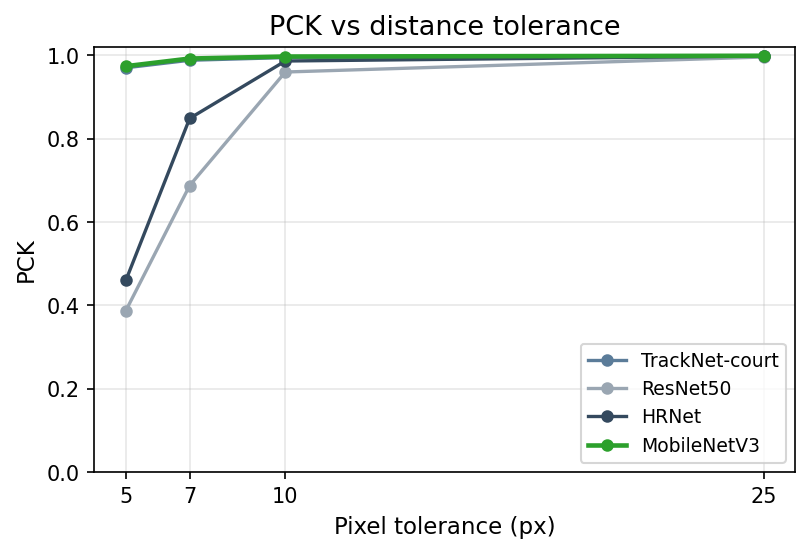
\includegraphics[width=\linewidth]{img/court_pck_curves.png}
    \caption{PCK across the tolerance sweep.}
    \label{fig:court-pck-curves}
  \end{subfigure}\hfill
  \begin{subfigure}{0.49\textwidth}
    \centering
    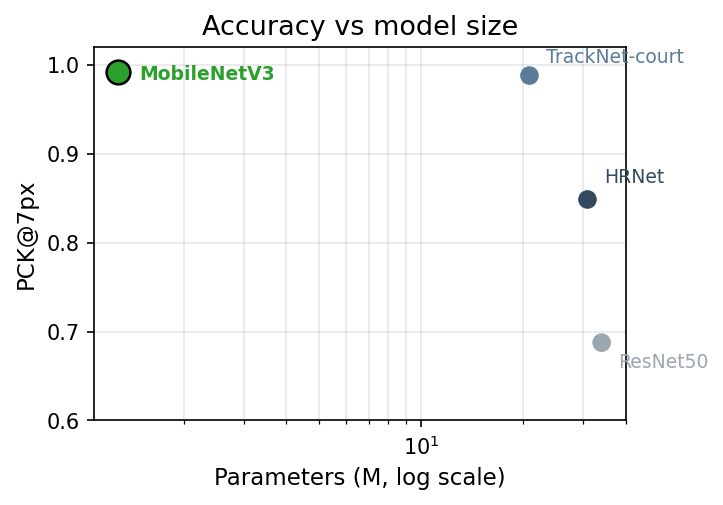
\includegraphics[width=\linewidth]{img/court_params_vs_pck.png}
    \caption{Accuracy against model size.}
    \label{fig:court-params}
  \end{subfigure}

  \vspace{0.7em}
  \begin{subfigure}{0.49\textwidth}
    \centering
    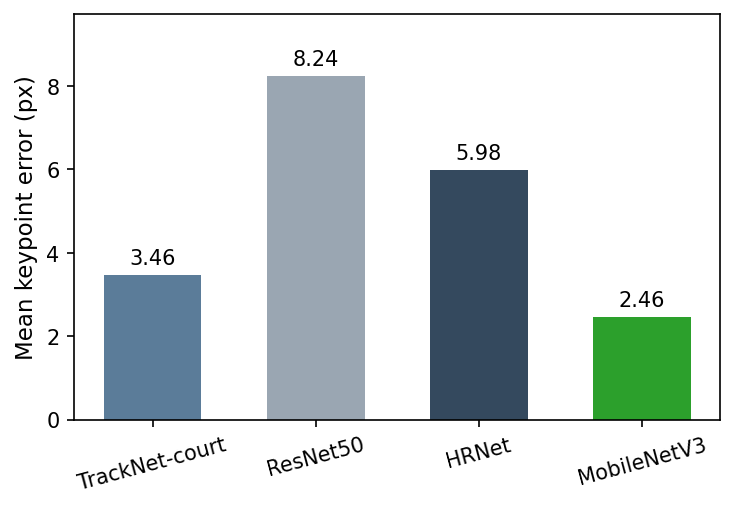
\includegraphics[width=\linewidth]{img/court_mean_kp_error.png}
    \caption{Mean keypoint error.}
    \label{fig:court-mae}
  \end{subfigure}\hfill
  \begin{subfigure}{0.49\textwidth}
    \centering
    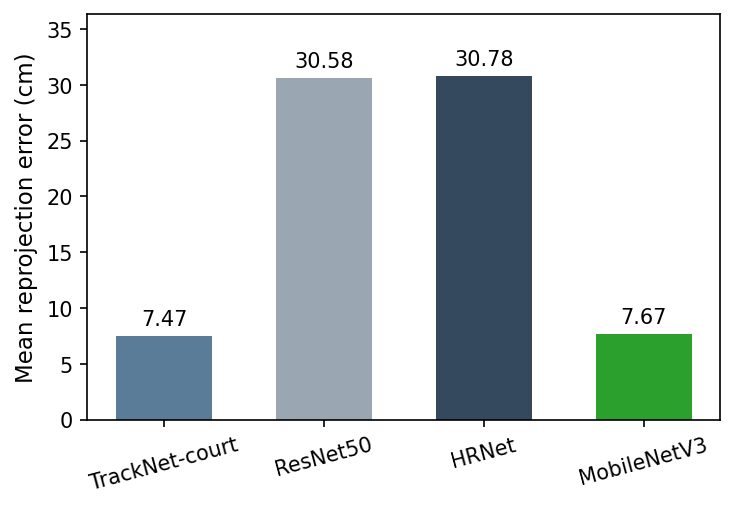
\includegraphics[width=\linewidth]{img/court_reproj_error.png}
    \caption{Mean court-plane reprojection error.}
    \label{fig:court-reproj}
  \end{subfigure}

  \caption{Four-model court-keypoint comparison; the plotted values are those of
    Table~\ref{tab:court-results}. (a)~The percentage of correct keypoints across
    the $\{5, 7, 10, 25\}$-pixel tolerance sweep, where the two output-stride-one
    models (TrackNet-court and MobileNetV3) lead at every tolerance while the two
    stride-four models (ResNet50 and HRNet) start far lower at five pixels and
    converge towards the others only as the tolerance widens. (b)~Accuracy at
    seven pixels against parameter count on a logarithmic axis, showing
    MobileNetV3 at the favourable corner, the smallest model at the top accuracy.
    (c)~Mean keypoint error and (d)~mean court-plane reprojection error per
    model, on both of which MobileNetV3 and TrackNet-court are far ahead of the
    two stride-four models.}
  \label{fig:court-comparison}
\end{figure}

The headline result is that MobileNetV3, by far the smallest of the four models,
is also the most accurate on every metric but one. It attains the best accuracy
at all four tolerances, including the most demanding five-pixel and seven-pixel
thresholds (0.974 and 0.992), the lowest mean keypoint error (2.46 pixels), the
joint-best homography success rate (0.999), and the highest throughput in the
comparison, while carrying 1.28 million parameters against the twenty to
thirty-four million of the others. Its median keypoint error is 1.45 pixels,
which shows that the bulk of its detections are localised to within a pixel or
two and that the mean is inflated by a small tail of harder frames; the same
holds for TrackNet-court, whose median error is 1.44 pixels. The single metric on
which MobileNetV3 does not lead is the mean reprojection error, where
TrackNet-court is marginally better at 7.47 centimetres against 7.67, a
difference too small to separate the two models in practice and far smaller than
the gap to the remaining two.

TrackNet-court, the dataset's own baseline architecture, is the second strongest
model and confirms that the task is well within reach of a heatmap detector: it
reaches 0.988 accuracy at seven pixels and the best reprojection error, but it
does so with sixteen times the parameters of MobileNetV3 and at the lowest
throughput of the four. ResNet50 and HRNet, despite being the two largest and
most capable backbones, are the two weakest court detectors at strict tolerance.
ResNet50 reaches only 0.388 accuracy at five pixels and 0.688 at seven, and HRNet
0.460 and 0.849, both far below the stride-one models, and their mean
reprojection errors of around thirty centimetres are four times worse. Their
accuracy recovers sharply as the tolerance widens, to 0.960 and 0.986 at ten
pixels and to near-parity with the others at twenty-five pixels, which indicates
that they place each keypoint in the right neighbourhood but not to the pixel
precision the strict thresholds demand. The reason for this pattern, which turns
on the output resolution of the models rather than on the capacity of their
backbones, is the subject of Section~\ref{sec:court-analysis}.

\begin{figure}[t]
  \centering
  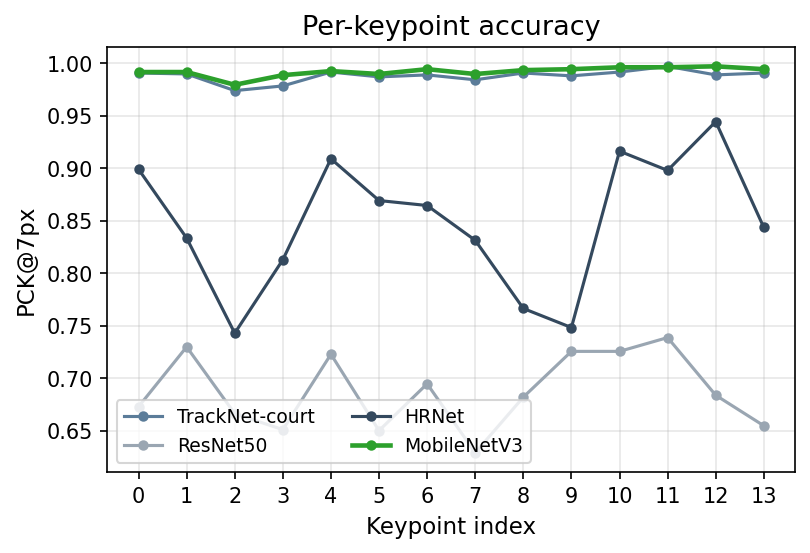
\includegraphics[width=0.85\textwidth]{img/court_per_keypoint_pck.png}
  \caption{Accuracy at seven pixels for each of the fourteen keypoints. The two
    stride-one models are uniformly high across all landmarks, whereas the two
    stride-four models are lower across every landmark rather than failing on any
    particular one, which is consistent with a resolution-limited rather than a
    landmark-specific cause.}
  \label{fig:court-perkp}
\end{figure}

The per-keypoint breakdown of Figure~\ref{fig:court-perkp} shows that no single
landmark dominates the error: the two strong models are uniformly accurate across
all fourteen keypoints, and the two weaker models are uniformly less accurate
rather than failing on a particular corner, which is consistent with a
resolution-limited rather than a landmark-specific cause. The homography success
rate is at least 0.995 for every model, so all four almost always produce enough
well-supported keypoints to register the court; the models are separated by the
precision of that registration, not by whether it can be obtained.
Figure~\ref{fig:court-qualitative} shows a qualitative example of the selected
model's output on a test frame, with the predicted keypoints close to the
ground-truth annotations across the visible court.

\begin{figure}[t]
  \centering
  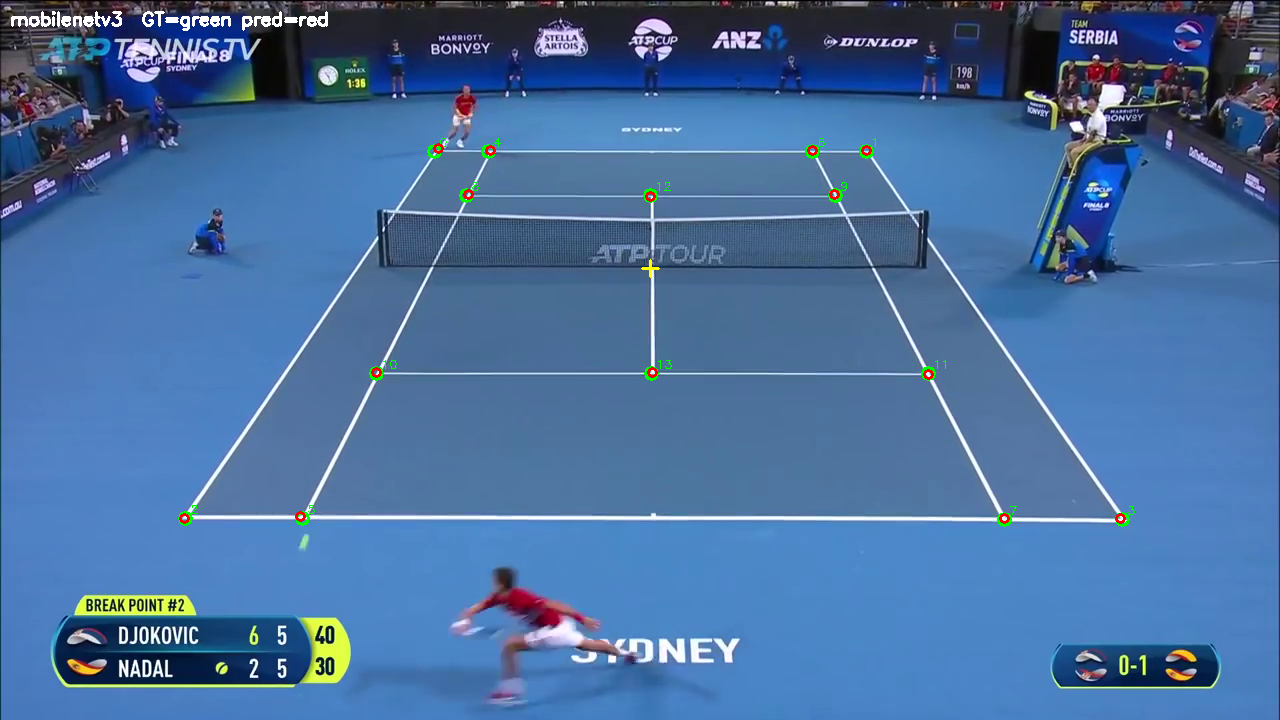
\includegraphics[width=0.8\textwidth]{img/court_overlay_mobilenetv3.png}
  \caption{Qualitative output of the selected MobileNetV3 model on a court test
    frame. Ground-truth keypoints are shown in green, the model's predictions in
    red, and the predicted court centre as a yellow cross. The predicted
    landmarks coincide closely with the ground truth across the court, including
    the far baseline where perspective foreshortening is strongest.}
  \label{fig:court-qualitative}
\end{figure}

These results answer RQ2. Among a heatmap baseline and three backbones of widely
differing size, the best accuracy against latency trade-off is given not by the
largest backbone but by the smallest, a 1.28-million-parameter MobileNetV3-Small
with a full-resolution decoder, which is the most accurate model at every
tolerance and the fastest in the comparison. Its mean court-plane reprojection
error of 7.67 centimetres, obtained on essentially every test frame, is small
relative to the scale of the court and the margins involved in a line call, so it
is reliable enough to drive the homography that the integrated system of
Chapter~\ref{ch:integrated} depends on, and it is the model selected for that
system.

\section{Analysis}
\label{sec:court-analysis}

The central finding of this chapter is that strict-tolerance accuracy on this
task is governed by the output resolution of the heatmap rather than by the
capacity of the backbone, and the four models divide cleanly along that line. The
two models that predict at output stride one, TrackNet-court and MobileNetV3,
emit a heatmap at the full $360 \times 640$ input grid, so that a single heatmap
cell corresponds to one input pixel and, after the factor-of-two rescaling to the
original frame, to about two pixels in the space where accuracy is measured. The
two models that predict at output stride four, ResNet50 and HRNet, emit a
$90 \times 160$ heatmap, so that one cell corresponds to four input pixels and to
about eight pixels in the original frame. The peak of a coarse heatmap can
therefore be no more precise than its cell, and although the sub-pixel refinement
of Section~\ref{sec:court-models} interpolates within a cell it cannot escape the
underlying lattice. A five-pixel tolerance is smaller than the eight-pixel
quantisation of the stride-four models, so even a perfectly centred prediction
frequently falls outside it, which is why ResNet50 and HRNet score so low at five
and seven pixels; once the tolerance widens past the quantisation step, at ten and
twenty-five pixels, a correctly identified cell almost always falls within
tolerance and the two models recover. The stride-one models, with a two-pixel
quantisation, sit comfortably inside even the five-pixel tolerance, which is why
they saturate the accuracy metric. The mean keypoint errors tell the same story
in pixel terms, around six and eight pixels for the stride-four models against
two and three for the stride-one models.

This explanation also resolves an apparent contradiction with the validation
figures used during training. The metric monitored for early stopping and
checkpoint selection was the accuracy at seven pixels measured in the resized
$360 \times 640$ input space, and on that metric all four models reach
comparable, high values, between 0.99 and 0.997. The seven-pixel tolerance in the
input space corresponds to a fourteen-pixel tolerance in the original frame, which
is wide enough to hide the quantisation penalty of the stride-four models;
measuring the test accuracy in the original space at seven pixels, the stricter
and more honest setting, is what exposes it. The lesson is methodological: the
space in which a pixel tolerance is applied must be stated alongside the number,
because the same nominal tolerance describes a different physical accuracy in the
input space and in the original space, and the input-space monitoring metric
flattered the coarse models.

It follows that the comparison is not a refutation of the larger backbones as
feature extractors but of the particular stride-four heads used here, and in the
case of HRNet of a head that does not exploit the backbone's defining
high-resolution branch. A fairer test of ResNet50 and HRNet would attach a decoder
that restores the full resolution, as the U-Net decoder does for MobileNetV3, and
their accuracy would be expected to rise accordingly. The practical conclusion for
this thesis is nonetheless robust: a lightweight, full-resolution model already
saturates the accuracy this task requires while costing a fraction of the
parameters and running fastest, so there is no accuracy argument for paying the
size and latency of the heavier models, and the small-backbone choice is the right
one for a deployable system.

Two further points qualify the results. First, the mean reprojection error in
centimetres should be read as an indicative geometric figure rather than an exact
one, because of how it is computed: ground-truth keypoints are projected through
the homography that was fitted to the predicted keypoints, so the number combines
the accuracy of the keypoints with the quality of the homography fit in a single
quantity, and a maximum reprojection error of well over a metre on the worst
frames, even for the strong models, reflects the occasional frame on which a
degenerate or poorly conditioned fit projects points far from their true
positions. The success rate and the mean error together, rather than either
alone, characterise the registration. Second, the court-centre channel that every
model emits is supervised during training but is not scored at evaluation, because
no ground-truth target for it is constructed in the evaluation loop; its accuracy
is therefore reported as not evaluated, and the channel serves only as an
auxiliary training signal and as an input to the geometric centre used elsewhere.

A local Hough-line refinement of the detected keypoints, which snaps each
prediction towards the nearest painted court line, was also explored as an
optional post-processing step. On the selected model it reduced the accuracy and
the throughput while changing the reprojection error only marginally, so it offers
no clear benefit at the operating point reached here and was not adopted for the
integrated system. Finally, the six excluded test records noted in
Section~\ref{sec:court-task} are a reminder that public datasets carry annotation
noise: they were found by a manual audit of the ground truth, and excluding them
prevents a handful of geometrically impossible annotations from distorting the
test metrics. Their identifiers are recorded in the project so that the exclusion
is reproducible.

In summary, the court comparison answers RQ2 by selecting a 1.28-million-parameter
MobileNetV3-Small model that is the most accurate of the four at every tolerance,
registers the court to within about eight centimetres on essentially every frame,
and runs fastest, and by showing that the accuracy ceiling on this task is set by
the heatmap output resolution rather than by backbone capacity. The selected model
provides the court geometry for the integrated system of
Chapter~\ref{ch:integrated}, where its homography projects the tracked ball and
the detected bounce into the court plane for the in-or-out line call.
